\section{}

\subsection{a) Suitable solutioning temperature and extent of the heat treatment window, and b) primary ageing temperature for new alloy}

To obtain a plot that can be used to find the solution temperature and treatment window, a calculation using \textit{One axis} with the following compositions was used:

\begin{table}[h]
  \centering
  \begin{tabular}{rrrrrrr}
    \multicolumn{1}{c}{x$_{Al}$} & \multicolumn{1}{c}{x$_{Ta}$} & \multicolumn{1}{c}{x$_{Cr}$} & \multicolumn{1}{c}{x$_{Re}$} & \multicolumn{1}{c}{x$_{W}$} & \multicolumn{1}{c}{x$_{Co}$} \\ \hline \hline
    18 & 2.24 & 0.2 & 0.5 & 0.5 & 15
  \end{tabular}
  \caption{Molar fraction composition of the Ni-Al-Ta-Cr-Re-W-Co alloy.}
  \label{tab:tab06}
\end{table}

\begin{figure}[h]
  \centering
    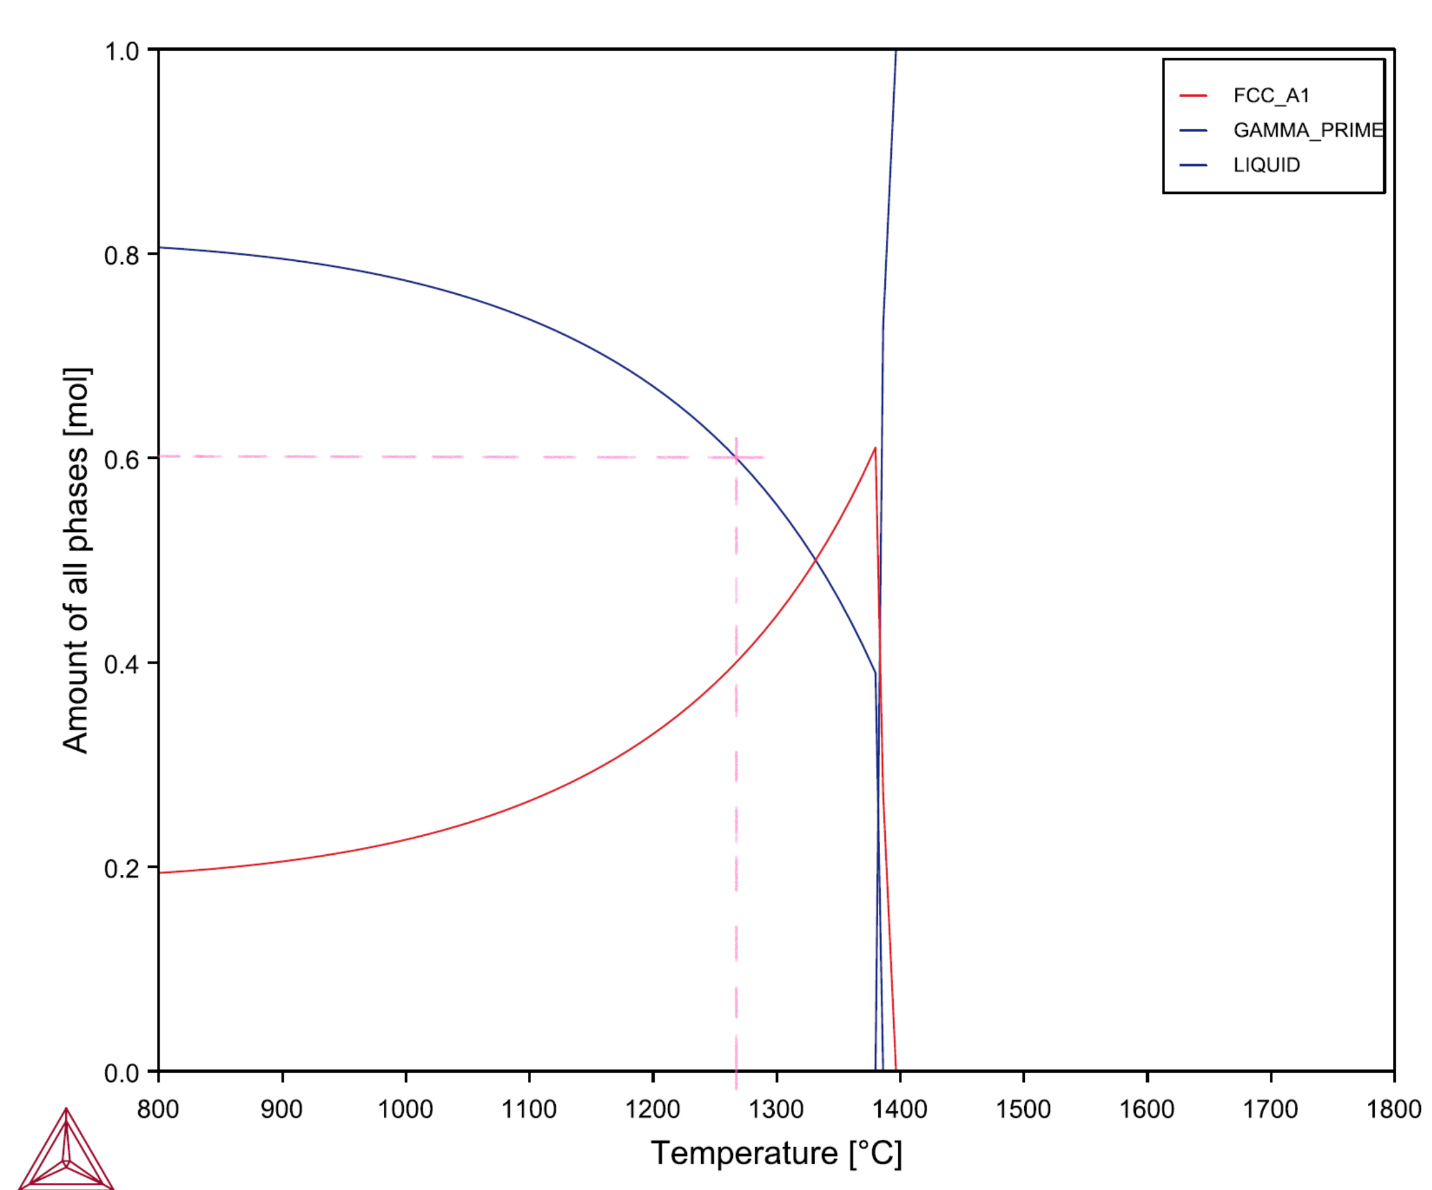
\includegraphics[width=0.95\textwidth]{graficas/Q4_02_1.png}
    \caption{\centering Amount of all phases as a function of temperature. \\
    \textit{Source: diagram generated with ThermoCalc \citep{thermocalc}.}}
    \label{fig:diagram05}
\end{figure}

\newpage
\textbf{a)} In  figure \ref{fig:diagram05} the amount of all phases is plotted as a function of temperature for the alloy system Ni-Al-Ta-Cr-Re-W-Co. It shows that the $\gamma'$ curve starts at a composition near $0.8$ value and decreases as the temperature increases, reaching a composition of value $0$ around $1388$°C. The temperature where the composition of the $gamma'$ phase becomes zero is the solutioning temperature. 

The liquid curve corresponds to an approximate temperature of $1380$°C, this temperature corresponds to the solidus temperature, where the liquid phase begins to form. 

The hear treatment window corresponds to de window that exists between the solutioning temperature, $1388$°C, to the solidus temperatures, $1380$°C, which gives a window of approximately $8$°C; so in this range of temperature the $\gamma'$ can be dissolved without partial melting of the alloy.

\textbf{b)} The primary ageing temperature is found at a $\gamma'$ fraction of 0.60, which corresponds to a temperature of approximately $1270$°C, as it is shown in figure \ref{fig:diagram05}. This is temperature at which a stable amount of precipitate can form and strengthen the alloy.